\documentclass{article}
\usepackage {inputenc, fullpage, listings, amsmath, graphicx, wasysym}

\parindent 0pt

\title{%
   CSc 320: Foundations of Computer Science (Summer 2022)\\
    \Large Alex Holland\\
    Assignment 2\\
    }
\date{}

\begin{document}

\maketitle

{\bf Question 1}\\
We want to show that given any regular language $L$, $L^+$ is regular. We can do this by taking a DFA $D$ that recognizes $L$ and constructing an NFA $N^+$. If DFA $D=(Q,\Sigma,\delta,q_0,F)$, then by definition $L^+=L^*-\epsilon$. Thus the empty string $\epsilon$ is not contained within $L$ or $L^+$. Every element in $L^+$ is accepted by $D$ since $L^+$ contains at least one combination of strings that are already in $L$. If we create a DFA with a defined start and accept state such as $q_1$ and $q_2$ respectively, we can introduce an $\epsilon$ for the $N^+$ that goes from $q_2$ to $q_1$. Note that this transition will work for all DFA's to NFA's with states between $q_1$ and $q_2$. 

\begin{center}
    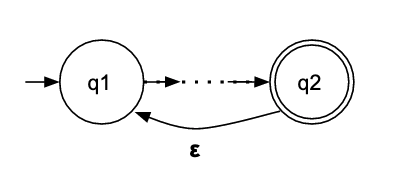
\includegraphics[width=0.6\textwidth]{1.png}
\end{center}

Every element of $L^+$ contains elements of L, we have $N^+$ that accepts $L^+$.  Therefore $L^+$ is a regular language.

\break
{\bf Question 2}\\
We can represent the states in the Transition Table:
\begin{center}
\begin{tabular}{||c c c c||} 
 \hline
 $\delta$ & $0$ & $1$ & $\epsilon$ \\ [0.5ex] 
 \hline\hline
 $q_1$ & $\{q_2\}$ &$\{q_2\}$ & $\emptyset$\\
 \hline
 $q_2$ & $\{q_5\}$ & $\{q_3\}$ & $\emptyset$\\
 \hline
 $q_3$ & $\{q_3\}$ & $\{q_3\}$ & $\emptyset$\\
 \hline
 $q_5$ & $\{q_6\}$ & $\{q_1\}$ & $\emptyset$\\
 \hline
 $q_6$ & $\{q_6\}$ & $\{q_6\}$ & $\emptyset$\\
 \hline
 $q_7$ & $\{q_2\}$ & $\{q_2\}$ & $\emptyset$\\
 \hline
\end{tabular}
\end{center}
The states, start state, and final states are the same for the equivalent NFA $A_N$.\\ 
Thus, $Q_N=Q_D$, $q_N=q_D$, $F_N=F_D$


\bigskip
{\bf Question 3}\\
Following the construction presented in class, given NFA $A_N = (Q_N,\Sigma,\delta_N,q_N,F_N)$ we can prove that for every NFA there exists an equivalent DFA.
\begin{comment}
$Q_D\subseteq P(Q_N)=\{\{q_0\},\{q_1\},\{q_2\},\{q_3\}, \{q_0,q_1\}, \{q_0, q_2\}, \{q_0, q_3\}, \{q_1, q_2\}, \{q_1, q_3\},$\\ $\{q_2, q_3\}, \{q_0, q_1, q_2\}, \{q_0, q_1, q_3\}, \{q_1, q_2, q_3\}, \{q_0, q_1, q_2, q_3,\}\}$
\end{comment}


\begin{center}
\begin{tabular}{||c c c||} 
 \hline
 $\delta_N$ & $a$ & $b$ \\ [0.5ex] 
 \hline\hline
 $\emptyset$ &  $\emptyset$ & $\emptyset$ \\
 \hline
 $\{q_0\}$ & $\{q_2,q_3\}$ & $\{q_1,q_2\}$ \\
 \hline
 $\{q_1\}$ & $\{q_3\}$ & $\emptyset$ \\
 \hline
 $\{q_2\}$ & $\{q_2,q_3\}$ & $\{q_2\}$ \\
 \hline
 $\{q_3\}$ & $\emptyset$ & $\emptyset$ \\
 \hline
 $\{q_0,q_1\}$ & $\{q_2,q_3\}$ & $\{q_1,q_2\}$ \\
 \hline
 $\{q_0,q_2\}$ & $\{q_2,q_3\}$ & $\{q_1,q_2\}$ \\
 \hline
 $\{q_1,q_3\}$ & $\{q_3\}$ & $\emptyset$ \\
 \hline
 $\{q_2,q_3\}$ & $\{q_2,q_3\}$ & $\{q_2\}$ \\
 \hline
 \hline
\end{tabular}
\end{center}



$Q_D\subseteq P(Q_N)=\{\emptyset, \{q_0\},\{q_1\},\{q_2\},\{q_3\}, \{q_0,q_1\}, \{q_0, q_2\}, \{q_0, q_3\}, \{q_1, q_2\}, \{q_1, q_3\},$\\ $\{q_2, q_3\}, \{q_0, q_1, q_2\}, \{q_0, q_1, q_3\}, \{q_0, q_2, q_3\}, \{q_1, q_2, q_3\}, \{q_0, q_1, q_2, q_3\}\}$\\


\begin{comment}
$Q_D=\{\emptyset, \{q_0\},\{q_1\},\{q_2\},\{q_3\}, \{q_0,q_1\}, \{q_0, q_2\}, \{q_1, q_3\}, \{q_2, q_3\}, \{q_0, q_1, q_2, q_3\}\}$\\
\end{comment}

$q_D$ is the start state and is $\{q_0, q_2\}$\\

The accept states in column $a$ are $F_D=\{q_2, q_3\}, \{q_3\}$


\bigskip
{\bf Question 4}\\
$L_1=\{wa|w\in\{a,b\}^*\}\cup\{ \epsilon \}$ is not recognized by A. Since $\epsilon$ is not accepted. E.g. aba$\epsilon$\\

$L_2=L((a \cup b)^*a)$ is recognized by A. Since any number of a and b's is followed by an a is accepted. E.g. aba\\

$L_3=L((a \cup b)^*)$ is not recognized by A. Since if there is any number of a,b's is followed by a b, then the string is not accepted. E.g. ab\\

$L_4=L((a \cup b)^* \cup b)L(a)$ is recognized by A. Since any number of a,b's is followed by b, followed by a is accepted. E.g. aba\\

$L_5=\{wa|w\in\{a,b\}^*\}$ is recognized by A. Since any number of a,b's is followed by b. E.g. ababa\\

$L_6=\{wbaa|w\in\{a,b\}^*\}$ is recognized by A.\\



\bre
{\bf Question 5}\\
{\bf (a)}\\
In $L(R_1)$ any strings that start with any number of a and b's, follwed by any number of c's, followed by aa. 
E.g. $abccaa, \; bbbcaa, \; aa$.\\

{\bf (b)}\\
State diagram for $M_1$ with $L(R_1) = L(M_1)$\\
The red circle indicates the portion: $(ab \cup ba)^*$\\
The blue circle indicates the portion: $(c)^*$\\
The green circle indicates the portion: $aa$\\
\begin{center}
    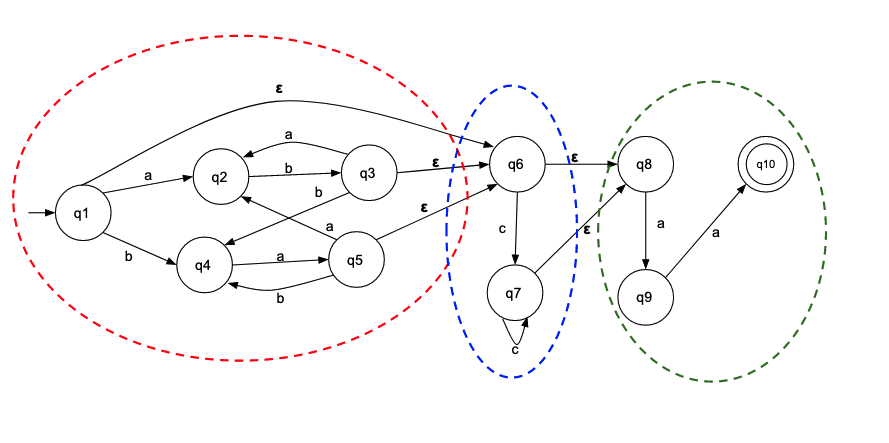
\includegraphics[width=0.95\textwidth]{5.png}
\end{center}

{\bf Question 6}\\
With the following GNFA, we want to determine the state diagram after ripping out state $q_r$
\begin{center}
    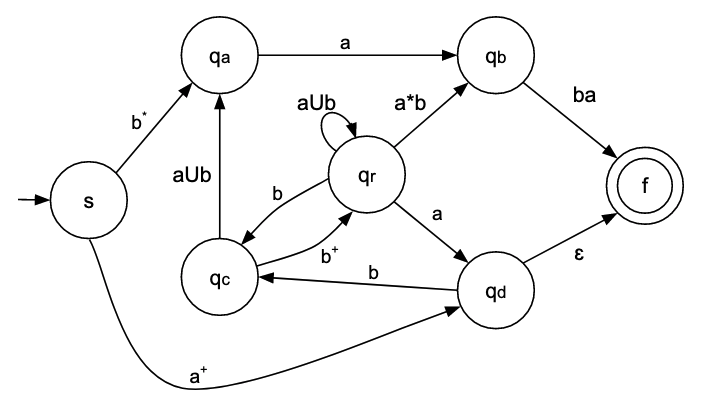
\includegraphics[width=0.6\textwidth]{6-1.png}
\end{center}
The state that goes into $q_r$ is $q_c$. The states that go out of $q_r$ is $q_b$, $q_c$, and $q_d$.\\
The transitions from $q_c$ to $q_d$ can be done by going through $b^+ \rightarrow$ $a \cup b$ (any number of times) $\rightarrow a$.\\
The transitions from $q_c$ to $q_c$ can be done by goring through $b^+ \rightarrow$ $a \cup b$ (any number of times) $\rightarrow b$\\
The transitions from $q_c$ to $q_b$ can be done by goring through $b^+ \rightarrow$ $a \cup b$ (any number of times) $\rightarrow a^*b$\\
\begin{center}
    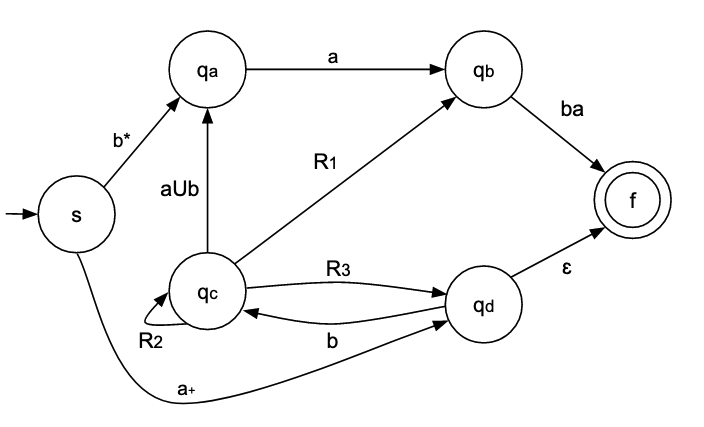
\includegraphics[width=0.6\textwidth]{6.png}
\end{center}
\begin{center}
    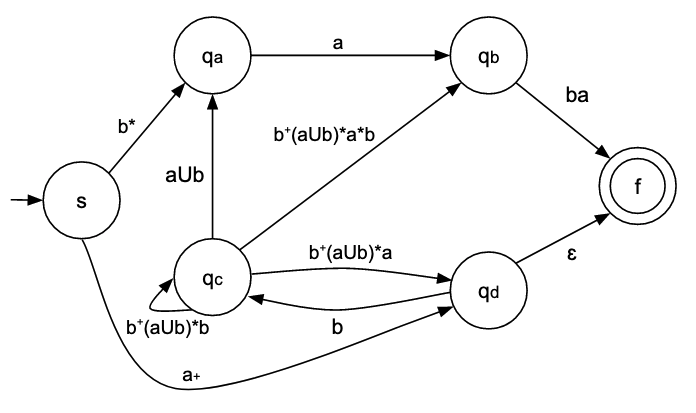
\includegraphics[width=0.6\textwidth]{6-2.png}
\end{center}
after ripping out $q_r$ we get that $R_1=b^+(a \cup b)^*a^*b$, $R_2= b^+(a \cup b)^*b$, and $R_3=b^+(a \cup b)^*a$

\end{document}
